\section{Scale and Conformal Symmetry (Concluded)}

\subsection{1/2/3-point correlation functions}
In principle, the correlation functions could be any function. But the symmetries actually constrain the functional form, and reduce the parameter dependence. 

Let $\Delta$ be the operator dimension. We had that the correlation functions depended just on the local operators $\phi(0)$ ($\Delta = \frac{D-2}{2}$), $\nabla_a \phi(0)$ ($\Delta = \frac{D-2}{2} + 1$), $\nabla_a\nabla_b\phi(0)$ ($\Delta = \frac{D-2}{2} + 2$), and the coefficients $C_{IJK}$. Finding these numbers is analogous to finding the spectrum of a Hamiltonian in a quantum mechanics problem.

How do we organize the contributing terms? Roughly the correlations scale in inverse $\Delta$, so the ones with larger $\Delta$ are less important and we can organize starting from smaller $\Delta$.

Looking at the dimensions of $\phi(x)$, we have that $\Delta_\phi = \frac{D-2}{2} + \eta$ and that $\Delta_{\phi^2} = D - 2 + \delta_{\Delta_{\phi^2}}$.

Besides a brute-force numerical calculation (which involves an infinite number of integrations), an $\e$-expansion is the only meaningful quantitative way to extract meaningful information about the problem (this is as far as analytical techniques go...). What about other approaches? Here we have assumed we have gone right to the fixed point. Suppose we take $\e = 1$, so the $\e$-expansion isn't useful; can we do anything in this scenario? We should develop our ideas about conformal symmetry even more. We don't have to go and solve the functional integral, because the Gaussian technique fails when the dimension is far from $4$. We consider the \emph{operator product expansion}.

\subsection{Operator Product Expansion}
This method gives us an equation of motion of sorts. If we take the product of two primary operators, this can be written as a sum over local operators:
\begin{equation}
    O_I(x_1)O_J(x_2) = \sum_K C_{IJK}(x_1 - x_3, x_2 - x_3, \dpd{}{x_3})O_K(x_3)
\end{equation}
This is analogous to having a complete set of states in quantum mechanics (and this is indeed how the above expansion is proven to exist).

Let us write the above in a slightly less general way:
\begin{equation}
    O_I(x_1)O_J(x_2) = \sum_K C_{IJK}(x_1 - x_2, \dpd{}{x_2})O_K(x_2)
\end{equation}
Now, the coefficients in this sum depend on the difference of coordinates as well as derivatives.

What's nice about this? If we take expectation values of both sides, on the LHS we have a two-point function and on the RHS we have one-point functions (for which th expectation values are zero, for the most part... the one that is nonzero is the constant/unit operator), so:
\begin{equation}
    \frac{\Delta_{IJ}}{\abs{x_1 - x_2}^{2\Delta_I}} = C_{IJ\II}(x_1 - x_2, 0).
\end{equation}
And we can see that the expansion is consistent with what we know about one and two-point functions so far. Beyond this, we can multiply the LHS by some other operator and take the expectation value; then we have the expectation value of a 3-point function on the LHS, and the sum of expectation values of 2-point functions on the RHS. Doing so, we get:
\begin{equation}
    \frac{C_{IJK}}{\abs{x_1 - x_2}^{\Delta_I + \Delta_J - \Delta_J}\abs{x_2 - x_3}^{\Delta_J + \Delta_K - \Delta_I}\abs{x_3 - x_1}^{\Delta_K + \Delta_I - \Delta_J}} = C_{IJK}(x_1 - x_2, \dpd{}{x_2})\frac{1}{\abs{x_2 - x_3}^{2\Delta_K}}
\end{equation}
If people tell you they are working on CFT, then they are basically using the operator product expansion, and then trying to calculate the different coefficients and the like.

So, we can use these equations to try to solve for the spectral data $C_{IJK}$; then, there are also some consistency requirements.

\subsection{4-point correlation function}
We now consider the expectation value of a 4-body operator; the 4-point correlation function. Here, the symmetries become less useful for trying to constrain the functional form. The four-point function can depend on the numbers:
\begin{equation}
    u = \frac{(x_1 - x_2)^2(x_3 - x_4)^2}{(x_1 - x_3)^2(x_2 - x_4)^2}, \quad v = \frac{(x_2 - x_3)^2(x_1 - x_4)^2}{(x_1 - x_3)^2(x_2 - x_4)^2}
\end{equation}
and unfortunately the symmetries tell us nothing about how the functions actually depend on these numbers; the general form of the four-point function is:
\begin{equation}
    \avg{\phi(x_1)\phi(x_2)\phi(x_3)\phi(x_4)} = \frac{g(u, v)}{\abs{x_1 - x_2}^{2\Delta_\phi}\abs{x_3 - x_4}^{2\Delta_\phi}}
\end{equation}
If we then diagramatically impose some constraints/that certain forms of the 4-point function must be equivalent:
\begin{figure}[htbp]
    \centering
    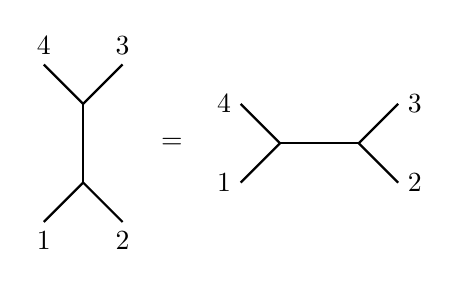
\begin{tikzpicture}[scale=0.5]
        \draw[thick] (0, 0) -- (0, 2);
        \draw[thick] (0, 2) -- (1, 3);
        \draw[thick] (0, 2) -- (-1, 3);
        \draw[thick] (0, 0) -- (-1, -1);
        \draw[thick] (0, 0) -- (1, -1);
        \node[below] at (-1, -1) {$1$};
        \node[below] at (1, -1) {$2$};
        \node[above] at (1, 3) {$3$};
        \node[above] at (-1, 3) {$4$};

        \node[] at (2.25, 1) {$=$};

        \draw[thick] (5, 1) -- (7, 1);
        \draw[thick] (5, 1) -- (4, 2);
        \draw[thick] (5, 1) -- (4, 0);
        \draw[thick] (7, 1) -- (8, 2);
        \draw[thick] (7, 1) -- (8, 0);
        \node[left] at (4, 0) {$1$};
        \node[right] at (8, 0) {$2$};
        \node[right] at (8, 2) {$3$};
        \node[left] at (4, 2) {$4$};
    \end{tikzpicture}
    \caption{Diagrammatic constraint on 4-point function - known as crossing symmetry.}
    \label{fig-crossingsymmetry}
\end{figure}
this crossing symmetry imposes a constraint on the operator expansion. In particular, we first consider that:
\begin{equation}
    \avg{\phi(x_1)\phi(x_2)\phi(x_3)\phi(x_4)} \sim \sum_k C_{IJK}C_{IJK}\ldots \sim \sum_K(C_{\phi\phi K})^2\ldots
\end{equation}
Then the crossing symmetry enforces:
\begin{equation}
    \sum_K(C_{\phi\phi K})^2[\text{stuff} - \text{stuff}] = 0
\end{equation}
and then we can ask when this has a consistent solution. By this constraint, we can find an allowed/disallowed region (where the plot is parameterized by the dimension of $\phi$ and $\phi^2$), as shown in Fig \ref{fig-montecarloplot}.

\begin{figure}[htbp]
    \centering
    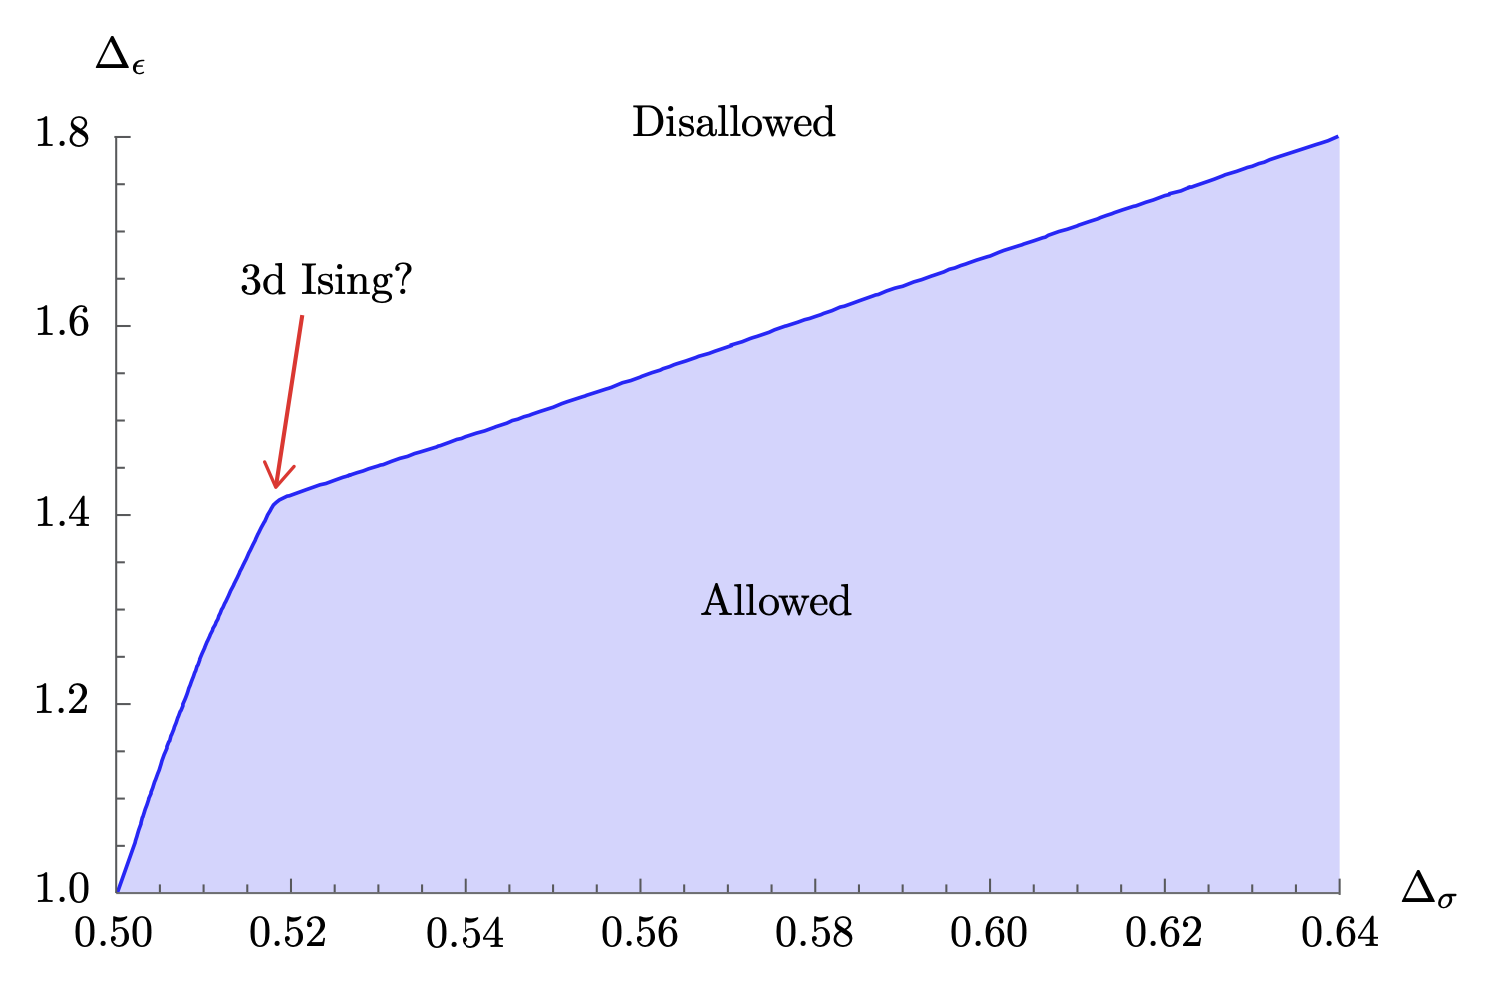
\includegraphics[scale=0.4]{Images/fig-montecarloplot.png}
    \caption{Allowed/Disallowed regions of the dimensions $\Delta_\sigma = \Delta_\phi$ and $\Delta_\e = \Delta_{\phi^2}$ as solved for by Monte Carlo. Figure reproduced without permission from ``TASI Lectures on the Conformal Bootstrap'' by David Simmons-Duffin.}
    \label{fig-montecarloplot}
\end{figure}

A more sophisticated computation (using what is known as the conformal bootstrap) yields Fig \ref{fig-CFTbootstrapplot}.

\begin{figure}[htbp]
    \centering
    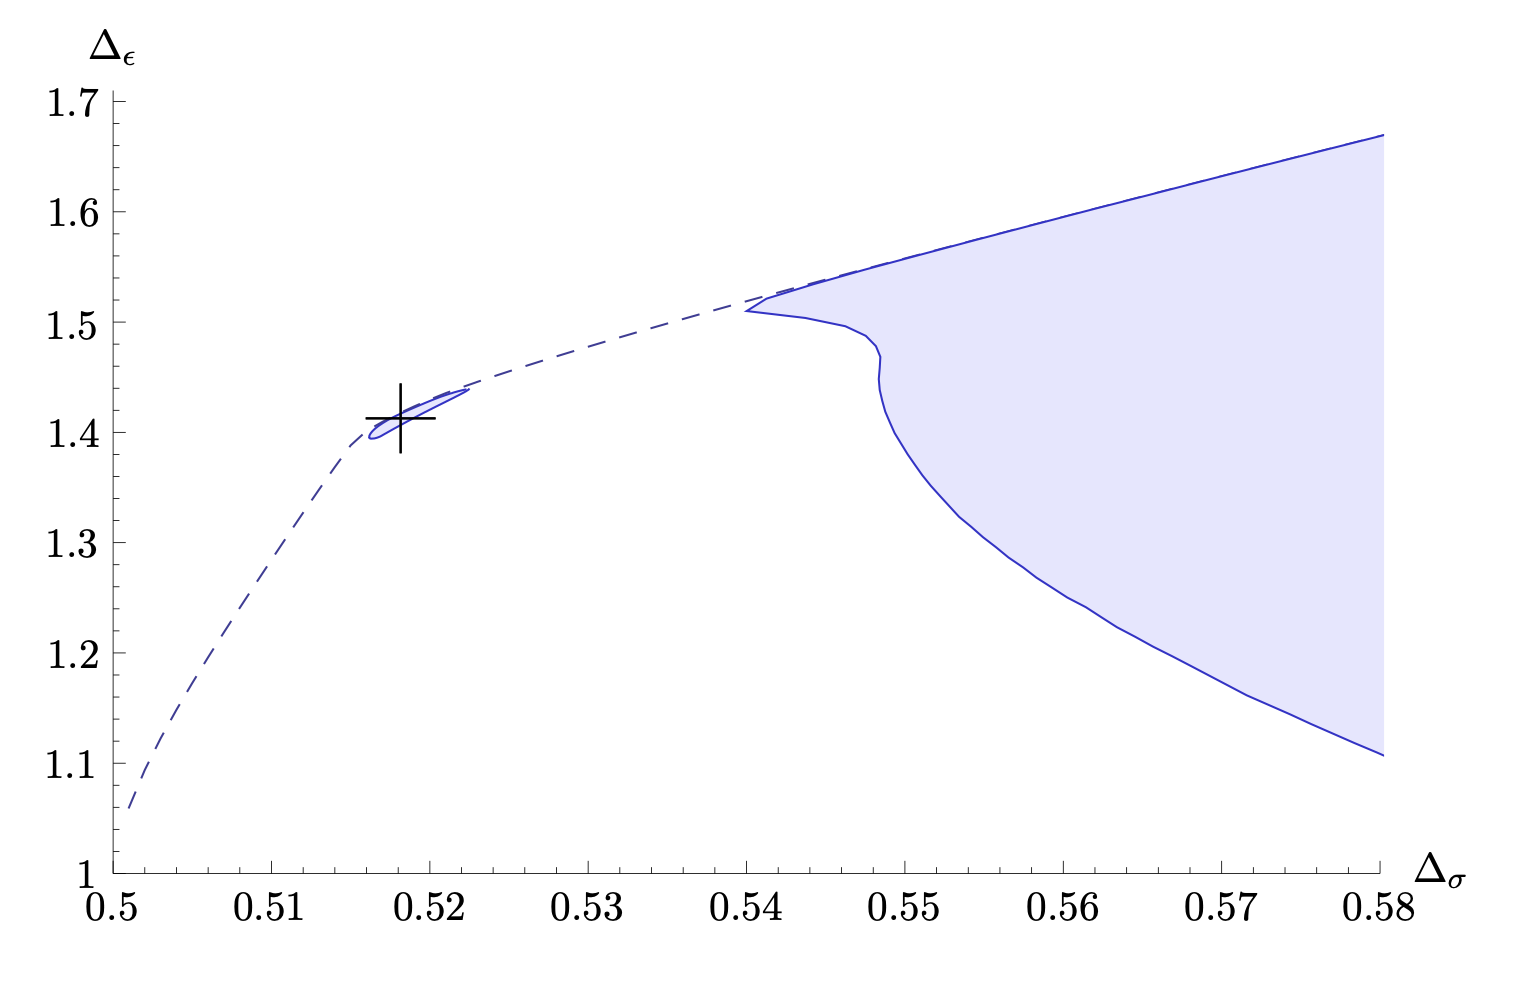
\includegraphics[scale=0.4]{Images/fig-CFTbootstrapplot.png}
    \caption{Allowed/Disallowed regions of the dimensions $\Delta_\sigma = \Delta_\phi$ and $\Delta_\e = \Delta_{\phi^2}$ as determined by the conformal bootstrap method. Figure reproduced without permission from ``TASI Lectures on the Conformal Bootstrap'' by David Simmons-Duffin.}
    \label{fig-CFTbootstrapplot}
\end{figure}

Here we can still see the ``Ising corner'' still persists, and shrinks to a small island. The accuracy we get here is something like six decimal places for critical exponents. For all intents and purposes, this procedure is an exact solution to the 3D Ising model. For $D = 3$, we find the dimensions:
\begin{equation}
    \Delta_\phi = 0.518151(6), \quad \Delta_{\phi^2} = 1.41264(6)
\end{equation}

This concludes the curriculum for this course. We can spend some of the rest of the time left reviewing what we have done.

\subsection{$O(N)$ model}
We consider a $D$-dimensional lattice, on which live $N$ component spin vectors.

\begin{equation}
    \hat{\sigma}(x) = (\sigma^1(x), \sigma^2(x), \ldots, \sigma^N(x))
\end{equation}
the spins are normalized:
\begin{equation}
    \sum_{a=1}^N (\sigma^a(x))^2 = 1.
\end{equation}
The Hamiltonian will have a term that wants neighbouring spins to align, and a magnetic field that wants to align the spins in a certain way:
\begin{equation}
    H = -J\sum_{x, i}\hat{\sigma}(x)\cdot \hat{\sigma}(x + i) - \v{B} \cdot \sum_x \hat{\sigma}(x)
\end{equation}
The partition function is given by:
\begin{equation}
    Z = \prod_x \int dn^a(x) e^{-H/k_B T}
\end{equation}
now in general we do not know how to do this integral. Nevertheless, there is our model written down! Now, we have to decide on an approach. Next time, we will decide on which approach to take.